\documentclass[10pt]{article}
\usepackage[margin=.7in]{geometry}\usepackage{tikz,hyperref}
\setlength{\parindent}{0pt}\setlength{\parskip}{7pt}
\begin{document}
\textbf{Normalization source attribution correction}\hfill2026-10-31\\T-1177. Producer correction and replay; independent fidelity review pending.

Four recent packets copied the first 61 lines of \texttt{projective\_law\_gate.rs}. Those excerpts contain none of \texttt{choose}, \texttt{transform} or \texttt{map\_divisor}. The original loop packet bound \texttt{genus2\_model\_gate.rs}; its current full-file hash still matches the original record. The defect is source attribution and excerpt selection, not a demonstrated canonical-source change.

Affected packets, preserved unchanged:\\
\texttt{coefficient-array-storage}; \texttt{coefficient-traversal}\\
\texttt{traversal-polynomial-composition}; \texttt{scale-trim-storage}.\\
Use this correction's named canonical excerpts and source map for source review.

\begin{center}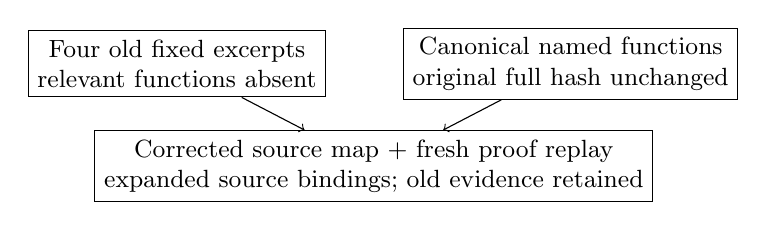
\begin{tikzpicture}[every node/.style={draw,align=center,font=\small}]
\node(a)at(0,0){Four old fixed excerpts\\relevant functions absent};
\node(b)at(5,0){Canonical named functions\\original full hash unchanged};
\node(c)at(2.5,-1.3){Corrected source map + fresh proof replay\\expanded source bindings; old evidence retained};
\draw[->](a)--(c);\draw[->](b)--(c);
\end{tikzpicture}\end{center}
The extractor records exact line ranges and full-file/function hashes. It requires one function-header match and balanced braces, and checks that the selected bodies contain no strings or comments that could confuse brace counting.

\begin{tabular}{lll}
Source & Function & Observed text correspondence\\\hline
Related gate & choose & matches after out $\to$ x\\
Related gate & transform & matches after scale\_inv $\to$ inv\\
Related gate & map\_divisor & absent\\
State collector & choose, transform & byte-identical\\
State collector & map\_divisor & matches after out $\to$ result
\end{tabular}

These are text comparisons, not compiler equivalence or independent semantic review. The mathematical statements and prior checks remain recorded, but the old excerpts do not provide the advertised source review material.

The unchanged Scale, Trim, Bridge, Controls and Readback modules were rebuilt in a fresh directory. The helper now also binds the intended canonical source, state collector, extraction script and source map. All five checks passed with unchanged input hashes. All 32 named axiom readbacks contain only standard Lean axioms. Existing compiled upstream dependencies remain within the trust boundary; this is a producer replay.

The additive packet includes this inspected PDF, editable SVG, structured status, full source snapshots, named excerpts and receipts. Earlier commentary suggesting canonical function movement is superseded by the source-attribution finding. Divisor-validity composition remains the next mathematical step. No scientific campaign, timing or cost ratio.
\end{document}
